%% History:
% Pavel Tvrdik (26.12.2004)
%  + initial version for PhD Report
%
% Daniel Sykora (27.01.2005)
%
% Michal Valenta (3.12.2008)
% rada zmen ve formatovani (diky M. Duškovi, J. Holubovi a J. Žďárkovi)
% sjednoceni zdrojoveho kodu pro anglickou, ceskou, bakalarskou a diplomovou praci

% One-page layout: (proof-)reading on display
%\documentclass[11pt,oneside,a4paper]{book}
% Two-page layout: final printing
\documentclass[11pt,twoside,a4paper]{book}   
%=-=-=-=-=-=-=-=-=-=-=-=--=%
% The user of this template may find useful to have an alternative to these 
% officially suggested packages:
\usepackage[czech, english]{babel}
\usepackage[T1]{fontenc} % pouzije EC fonty 
% pripadne pisete-li cesky, pak lze zkusit take:
%\usepackage[OT1]{fontenc} 
\usepackage[utf8]{inputenc}
\usepackage{cmap}
\usepackage{mathpazo}
\usepackage[final]{pdfpages}

%=-=-=-=-=-=-=-=-=-=-=-=--=%
% In case of problems with PDF fonts, one may try to uncomment this line:
%\usepackage{lmodern}
%=-=-=-=-=-=-=-=-=-=-=-=--=%
%=-=-=-=-=-=-=-=-=-=-=-=--=%
% Depending on your particular TeX distribution and version of conversion tools 
% (dvips/dvipdf/ps2pdf), some (advanced | desperate) users may prefer to use 
% different settings.
% Please uncomment the following style and use your CSLaTeX (cslatex/pdfcslatex) 
% to process your work. Note however, this file is in UTF-8 and a conversion to 
% your native encoding may be required. Some settings below depend on babel 
% macros and should also be modified. See \selectlanguage \iflanguage.
%\usepackage{czech}  %%%%%
%\usepackage[T1]{czech} %%%%[IL2] [T1] [OT1]
%=-=-=-=-=-=-=-=-=-=-=-=--=%

%%%%%%%%%%%%%%%%%%%%%%%%%%%%%%%%%%%%%%%
% Styles required in your work follow %
%%%%%%%%%%%%%%%%%%%%%%%%%%%%%%%%%%%%%%%
\usepackage{graphicx}
%\usepackage{indentfirst} %1. odstavec jako v cestine.

\usepackage{k336_thesis_macros} % specialni makra pro formatovani DP a BP
% muzete si vytvorit i sva vlastni v souboru k336_thesis_macros.sty
% najdete  radu jednoduchych definic, ktere zde ani nejsou pouzity
% napriklad: 
% \newcommand{\bfig}{\begin{figure}\begin{center}}
% \newcommand{\efig}{\end{center}\end{figure}}
% umoznuje pouzit prikaz \bfig namisto \begin{figure}\begin{center} atd.

\newcommand\TypeOfWork{Diplomová práce} \typeout{Diplomova prace}
\newcommand\StudProgram{Otevřená informatika, Magisterský}
\newcommand\StudBranch{Počítačové vidění a digitální obraz}
\newcommand\WorkTitle{Automatizovaná analýza částic v mikroskopických snímcích}
\newcommand\FirstandFamilyName{Bc. Jiří Palas}
\newcommand\Supervisor{doc. RNDr. Ing. Marcel Jiřina, PhD.}


% Pouzijete-li pdflatex, tak je prijemne, kdyz bude mit vase prace
% funkcni odkazy i v pdf formatu
\usepackage[
pdftitle={\WorkTitle},
pdfauthor={\FirstandFamilyName},
bookmarks=true,
colorlinks=true,
breaklinks=true,
urlcolor=black,
citecolor=black,
linkcolor=black,
unicode=true,
]
{hyperref}



% Extension posted by Petr Dlouhy in order for better sources reference (\cite{} command) especially in Czech.
% April 2010
% See comment over \thebibliography command for details.

\usepackage[square, numbers]{natbib}             % sazba pouzite literatury
\usepackage{url}
%\DeclareUrlCommand\url{\def\UrlLeft{<}\def\UrlRight{>}\urlstyle{tt}}  %rm/sf/tt
%\renewcommand{\emph}[1]{\textsl{#1}}    % melo by byt kurziva nebo sklonene,
\let\oldUrl\url
\renewcommand\url[1]{<\texttt{\oldUrl{#1}}>}




\begin{document}

%%%%%%%%%%%%%%%%%%%%%%%%%%%%%%%%%%%%%
% Zvolte jednu z moznosti 
% Choose one of the following options
%%%%%%%%%%%%%%%%%%%%%%%%%%%%%%%%%%%%%
\selectlanguage{czech}
%\selectlanguage{english} 

% prikaz \typeout vypise vyse uvedena nastaveni v prikazovem okne
% pro pohodlne ladeni prace


\iflanguage{czech}{
	 \typeout{************************************************}
	 \typeout{Zvoleny jazyk: čeština}
	 \typeout{Typ práce: \TypeOfWork}
	 \typeout{Studijní program: \StudProgram}
	 \typeout{Obor: \StudBranch}
	 \typeout{Jméno: \FirstandFamilyName}
	 \typeout{Název práce: \WorkTitle}
	 \typeout{Vedoucí práce: \Supervisor}
	 \typeout{***************************************************}
	 \newcommand\Department{Katedra kybernetiky}
	 \newcommand\Faculty{Fakulta elektrotechnická}
	 \newcommand\University{České vysoké učení technické v Praze}
	 \newcommand\labelSupervisor{Vedoucí práce}
	 \newcommand\labelStudProgram{Studijní program}
	 \newcommand\labelStudBranch{Obor}
}{
	 \typeout{************************************************}
	 \typeout{Language: english}
	 \typeout{Type of Work: \TypeOfWork}
	 \typeout{Study Program: \StudProgram}
	 \typeout{Study Branch: \StudBranch}
	 \typeout{Author: \FirstandFamilyName}
	 \typeout{Title: \WorkTitle}
	 \typeout{Supervisor: \Supervisor}
	 \typeout{***************************************************}
	 \newcommand\Department{Department of Computer Science and Engineering}
	 \newcommand\Faculty{Faculty of Electrical Engineering}
	 \newcommand\University{Czech Technical University in Prague}
	 \newcommand\labelSupervisor{Supervisor}
	 \newcommand\labelStudProgram{Study Programme} 
	 \newcommand\labelStudBranch{Field of Study}
}




%%%%%%%%%%%%%%%%%%%%%%%%%%    Poznamky ke kompletaci prace
% Nasledujici pasaz uzavrenou v {} ve sve praci samozrejme 
% zakomentujte nebo odstrante. 
% Ve vysledne svazane praci bude nahrazena skutecnym 
% oficialnim zadanim vasi prace.
%{
%\pagenumbering{roman} \cleardoublepage \thispagestyle{empty}
%\chapter*{Na tomto místě bude oficiální zadání vaší práce}
%\begin{itemize}
%\item Toto zadání je podepsané děkanem a vedoucím katedry,
%\item musíte si ho vyzvednout na studijním oddělení Katedry počítačů na Karlově náměstí,
%\item v jedné odevzdané práci bude originál tohoto zadání (originál zůstává po obhajobě na katedře),
%\item ve druhé bude na stejném místě neověřená kopie tohoto dokumentu (tato se vám vrátí po obhajobě).
%\end{itemize}
%\newpage
%}
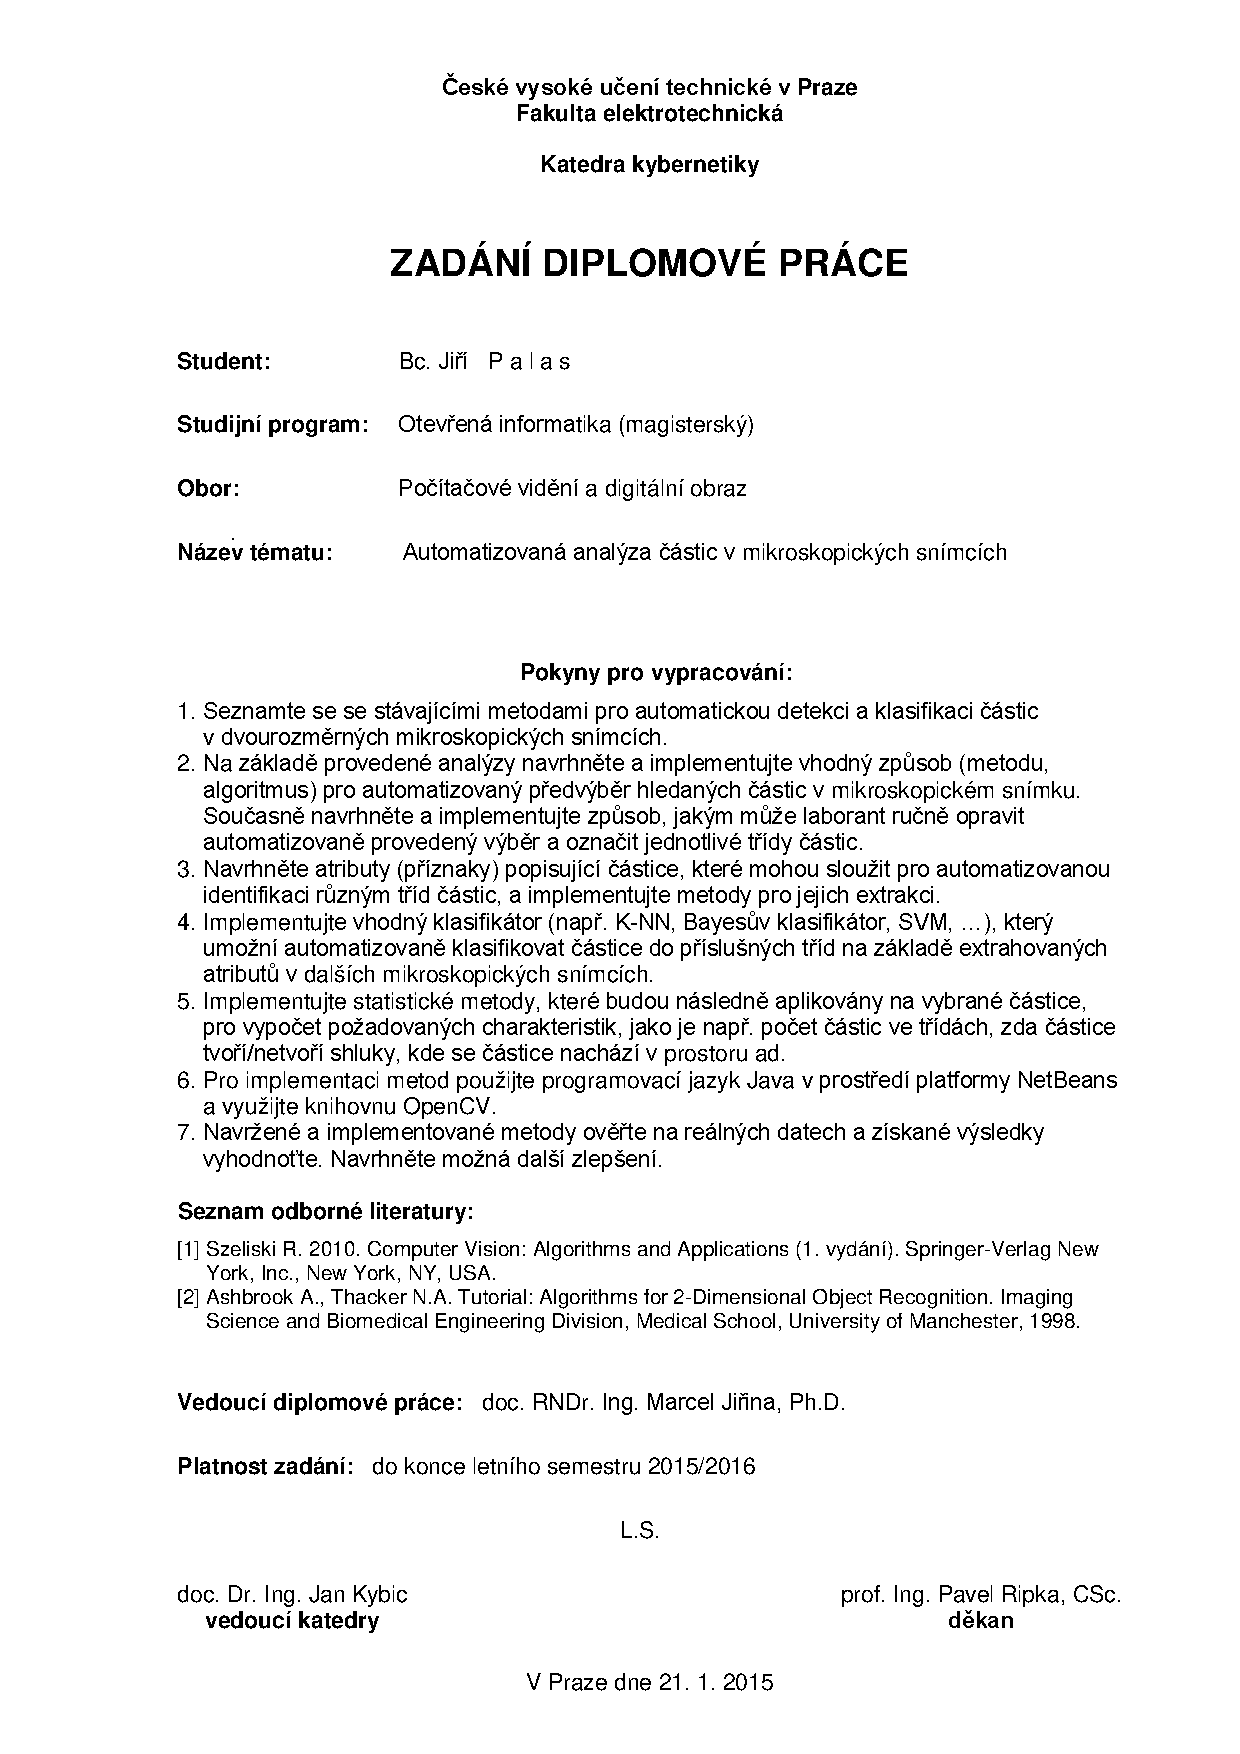
\includepdf[pages={1,{}}]{zadani.pdf}

%%%%%%%%%%%%%%%%%%%%%%%%%%    Titulni stranka / Title page 

\coverpagestarts

%%%%%%%%%%%%%%%%%%%%%%%%%%%    Podekovani / Acknowledgements 

\acknowledgements
\noindent
Na tomto místě bych rád poděkoval mamince za vaření obědů a večeří během krušných hodin psaní.


%%%%%%%%%%%%%%%%%%%%%%%%%%%   Prohlaseni / Declaration 

\declaration{V~Praze dne 11.\,5.\,2015}


%%%%%%%%%%%%%%%%%%%%%%%%%%%%    Abstract 
 
\abstractpage

Abstrakt v angličtině.

% Prace v cestine musi krome abstraktu v anglictine obsahovat i
% abstrakt v cestine.
\vglue60mm

\noindent{\Huge \textbf{Abstrakt}}
\vskip 2.75\baselineskip

\noindent
TODO Ještě nějak lépe přeformulovat

Tato práce si klade za cíl návrh a implementaci software zaměřeného na automatizovanou analýzu částic v mikroskopických snímcích. Práce se zabývá analýzou současných metod zpracování obrazu a strojového učení využitelnými pro automatizovanou detekci, klasifikaci a analýzu mikroskopických částic. Na jejím základě je navržen a implementován algoritmus pro automatizovanou detekci a klasifikaci částic. V rámci práce jsou navrženy a implementovány metody vizuální a interaktivní analýzu detekovaných a klasifikovaných částic.

%******************************  Obsah / Table of Contents 
\tableofcontents

%******************************  Seznam obrazku / List of Figures 
\listoffigures

%******************************  Seznam tabulek / List of Tables
\listoftables

%**************************************************************

\mainbodystarts
% horizontalní mezera mezi dvema odstavci
%\parskip=5pt
%11.12.2008 parskip + tolerance
%\normalfont
\fontsize{11pt}{15pt}\selectfont
\parskip=0.3\baselineskip plus 0.2\baselineskip minus 0.1\baselineskip

% Odsazeni prvniho radku odstavce resi class book (neaplikuje se na prvni 
% odstavce kapitol, sekci, podsekci atd.) Viz usepackage{indentfirst}.
% Chcete-li selektivne zamezit odsazeni 1. radku nektereho odstavce,
% pouzijte prikaz \noindent.


%*****************************************************************************
\chapter{Úvod}

\section{Motivace}
Popsat současný stav věci, 
Klíčové součásti: detekce, klasifikace, analýza

\section{Cíle}

\section{Přehled}

\section{Elektronová mikroskopie}
Krátký stručný popis jak to funguje co se tam 

\section{Data}
Popis dat (obrázků, snímků). Co v nich hledáme? Proč to hledáme?

% *****************************************************************************
\chapter{Dostupné metody}

\section{Detekce}
Krátká rešerše vybraných metod.

\section{Klasifikace}
Krátká rešerše vybraných metod.

\section{Analýza}

\chapter{Implementace}

\section{Detekce}
Popis použitého algoritmu detekce.

Metoda detekce kontur (přečíst a zpracovat):
Suzuki, S. and Abe, K., Topological Structural Analysis of Digitized Binary Images by Border Following. CVGIP 30 1, pp 32-46 (1985)

K implementaci této metody bylo využito OpenCV.

Co se detekovalo špatně během procesu a jak jsem to optimalizoval.
Jak vizualizuji výsledky detekce.

\section{Klasifikace}
\subsection{Výběr příznaků}
\subsection{Výběr klasifikátoru}
Popis použitého algoritmu klasifikace. Klasifikátor KNN. 
Proč jsem zvolil zrovna KNN a ne třeba SVM. Postup do klasifikátoru.
Nastavení parametrů
jak se přidávají data
Jak jsem se vypořádal s problémem registrace klasifikátoru k obrázku.
Jak jsem se vypořádal s problémem ukládání naučeného klasifikátoru.
Jak vizualizuji výsledky detekce.

\section{Analýza}
Popis navržených metod hierarchického shlukování.

\chapter{Výsledky}
Zde vyhodnocení použitých algoritmů na 10 testovacích obrázcích.
Použité obrázky. Do příloh ve velkém formátu.

\section{Detekce}
Vyhodnocení segmentace. Co se nedetekovalo a mělo detekovat

\section{Klasifikace}
Ukázat vstupní nastavení příkladů na kterých se naučí klasifikátor. Ukázat na pár snímcích jak to dopadlo. Plus vyhodnocení jak to dopadlo. Procentuální vyhodnocení úspěšnosti vybraného klasifikátoru.

\chapter{Závěr}
\section{Shrnutí práce}
Čeho jsem dosáhl.

\section{Další směřování}
Co by se dalo přidat nebo změnit.

%*****************************************************************************
% Seznam literatury je v samostatnem souboru reference.bib. Ten
% upravte dle vlastnich potreb, potom zpracujte (a do textu
% zapracujte) pomoci prikazu bibtex a nasledne pdflatex (nebo
% latex). Druhy z nich alespon 2x, aby se poresily odkazy.

% originally following specification for bibliography formating was used
%\bibliographystyle{abbrv}

% Here is an improvment by Petr Dlouhy (April 2010).
% It is mainly for supervisors who expect Czech fomrating rules for references
% Additional feature is live url addresses to sources from your pdf file
% It requires the file csplainnat.bst (included in this sample zipfile).

\bibliographystyle{csplainnat}

%bibliographystyle{plain}
%\bibliographystyle{psc}
{
%JZ: 11.12.2008 Kdo chce mit v techto ukazkovych odkazech take odkaz na CSTeX:
%\def\CS{$\cal C\kern-0.1667em\lower.5ex\hbox{$\cal S$}\kern-0.075em $}
\bibliography{reference}
}

% M. Dušek radi:
%\bibliographystyle{alpha}
% kdy citace ma tvar [AutorRok] (napriklad [Cook97]). Sice to asi neni  podle ceske normy (BTW BibTeX stejne neodpovida ceske norme), ale je to nejprehlednejsi.
% 3.5.2009 JZ polemizuje: BibTeX neobvinujte, napiste a poskytnete nam styl (.bst) splnujici citacni normu CSN/ISO.

%*****************************************************************************
%*****************************************************************************
\appendix


%*****************************************************************************
\chapter{Seznam použitých zkratek}

\begin{description}
\item[API] - Application Programming Interface 
\end{description}

%*****************************************************************************
\chapter{Obsah přiloženého CD}
V této kapitole naleznete obsah CD přiloženého k této diplomové práci.

\begin{itemize}
	\item readme.txt - popis obsahu CD s dalšími informacemi
	\item pattern/ - zdrojové kódy aplikace v jazyce Java
	\item text/
	\begin{itemize}
		\item src/ - zdrojový text v LaTeXu, včetně obrázků a šablon
		\item palasjir\_2015dip.pdf - text diplomové práce ve formátu PDF
	\end{itemize} 
\end{itemize}

\end{document}
